\begin{figure*}[t]
    \centering
    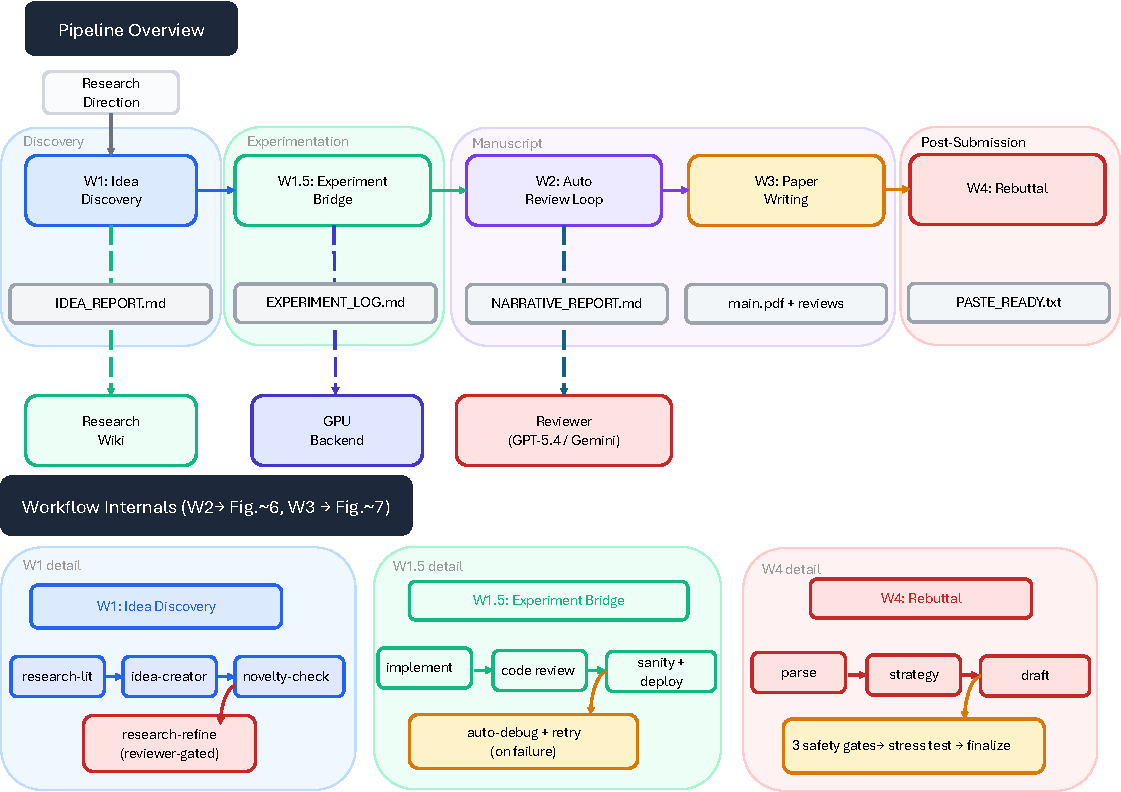
\includegraphics[width=0.95\textwidth]{figures/srcs/05_pipeline.pdf}
    \caption{\aris{} workflow library. \textbf{Top}: end-to-end composition of the five workflows and their artifact contracts, grouped into four research phases (Discovery, Experimentation, Manuscript, Post-Submission); dashed links denote reviewer feedback, GPU-triggered evidence collection, and wiki memory. \textbf{Bottom}: compressed internal structure for the workflows not otherwise expanded in the main text---W1 idea discovery (with reviewer-gated refinement), W1.5 experiment bridge (with code review and auto-debug fallback), and W4 rebuttal (with safety gates and stress test). W2 auto-review and W3 paper writing internals are detailed separately in Figures~\ref{fig:wf2} and~\ref{fig:wf3}.}
    \label{fig:pipeline}
\end{figure*}
